%%% exemplo de utilização da classe ita
%%%
%%%   por        fábio fagundes silveira   -  ffs [at] ita [dot] br
%%%              benedito c. o. maciel     -  bcmaciel [at] ita [dot] br
%%%              giovani volnei meinertz   -  giovani [at] ita [dot] br
%%%    	         hudson alberto bode       -  bode [at] ita [dot]br
%%%    	         p. i. braga de queiroz    -  pi [at] ita [dot] br
%%%    	         jorge a. b. gripp         -  gripp [at] ita [dot] br
%%%    	         juliano monte-mor         -  jamontemor [at] yahoo [dot] com [dot] br
%%%    	         tarcisio a. b. gripp      -  tarcisio.gripp [at] gmail [dot] com
%%%
%%%   versão para overleaf:
%%%   por           alejandro a. rios cruz - aarc.88@gmail.com
%%%                 saulo gómez            - sagomezs@unal.edu.co
%%%  importante: o texto contido neste exemplo nao significa absolutamente nada.  :-)
%%%              o intuito aqui eh demonstrar os comandos criados na classe e suas
%%%              respectivas utilizacoes.
%%%
%%%  tese.tex  2016-08-25
%%%  $headurl: http://www.apgita.org.br/apgita/teses-e-latex.php $
%%%
%%% italus
%%% instituto tecnológico de aeronáutica --- ita, sao jose dos campos, brasil
%%%                   http://groups.yahoo.com/group/italus/
%%% discussion list: italus {at} yahoogroups.com
%%%
%++++++++++++++++++++++++++++++++++++++++++++++++++++++++++++++++++++++++++++++
% para alterar o tipo de documento, preencher a linha abaixo \documentclass[?]{?}
%   \documentclass[tg]{ita}			= trabalho de graduacao
%   \documentclass[tgfem]{ita}	= para engenheiras
%   								msc     		= dissertacao de mestrado
%   								mscfem   		= para mestras
%   								dsc      		= tese de doutorado
%   								dscfem   		= para doutoras
%   								quali    		= exame de qualificacao
%   								qualifem 		= exame de qualificacao para doutoras
% para 'draft version'/'versao preliminar' com data no rodape, adicionar 'dv':
%   \documentclass[dsc, dv]{ita}
% para trabalhos em inglês, adicionar 'eng':
%   \documentclass[dsc, eng]{ita}
%		\documentclass[dsc, eng, dv]{ita}
%++++++++++++++++++++++++++++++++++++++++++++++++++++++++++++++++++++++++++++++
\documentclass[tg]{ita}    % ita.cls based on standard book.cls
% quando alterar a classe, por exemplo de [msc] para [msc, eng]) rode mais uma vez o botão build output caso haja erro
\usepackage{ae}
\usepackage{graphicx}
\usepackage{epsfig}
\usepackage{amsmath}
\usepackage{amssymb}
\usepackage{subfig}
\usepackage{multirow}
\usepackage{float}
\usepackage{amsthm}
\usepackage{url}         % formats url addresses properly
\usepackage{appendix}    % allows appendix section to be included
\usepackage{lscape}      % allows a page to be rendered in landscape mode
\usepackage{multicol}    % allows text in multi columns
\usepackage{cancel}      % needed to show canceled terms in equations
\usepackage{lettrine}
\usepackage{float}
\usepackage{placeins}
\usepackage[outputdir=latex.out]{minted}
\usepackage{prettyref}
\usepackage{flafter}  % put this in your pre-amble
\usepackage{tikz}
\usepackage{listings}

% \renewcommand\listingscaption{Código}
\renewcommand{\lstlistingname}{Código}% Listing -> Algorithm
\renewcommand{\lstlistlistingname}{List of \lstlistingname s}% List of Listings -> List of Algorithms
% \lstlistoflistings
\newcommand{\textunderscript}[1]{$_{\text{#1}}$}
\newrefformat{anex}{Anexo~\ref{#1}}
\newrefformat{cap}{Capítulo~\ref{#1}}
\newrefformat{lst}{Código~\ref{#1}}
\newrefformat{tbl}{Tabela~\ref{#1}}

% \newenvironment{code}{\captionsetup{type=listing, position=above}}{}
% Make ref autocomplete work.
\newcommand{\cref}[1]{\prettyref{#1}}

\usemintedstyle{friendly}

%HHHHHHHHHHHHHHHHHHHHHHHHHHHHHHHHHHHHHHHHHHHHHHHHHHHHHHHHHHHHHHHHHHHHHHHHHHHHHHHHHHHHHHHHHHHHHHHHHHHHHHHHHHHH
%\usepackage{subfigure}
%\usepackage{subfigmat}
%PACOTEFIGURAS_SE _ERRADO_ESXCLUIR_ACIMA
\usepackage{booktabs}
%PACOTETABELAS_SE _ERRADO_ESXCLUIR_ACIMA
%HHHHHHHHHHHHHHHHHHHHHHHHHHHHHHHHHHHHHHHHHHHHHHHHHHHHHHHHHHHHHHHHHHHHHHHHHHHHHHHHHHHHHHHHHHHHHHHHHHHHHHHHHHHH

%++++++++++++++++++++++++++++++++++++++++++++++++++++++++++++++++++++++++++++++
% Espaçamento padrão de todo o documento
%++++++++++++++++++++++++++++++++++++++++++++++++++++++++++++++++++++++++++++++
\onehalfspacing

%singlespacing Para um espaçamento simples
%onehalfspacing Para um espaçamento de 1,5
%doublespacing Para um espaçamento duplo

%++++++++++++++++++++++++++++++++++++++++++++++++++++++++++++++++++++++++++++++
% Identificacoes (se o trabalho for em inglês, insira os dados em inglês)
% Para entradas abreviadas de Professora (Profa.) em português escreva: Prof$^\textnormal{a}$.
%++++++++++++++++++++++++++++++++++++++++++++++++++++++++++++++++++++++++++++++
\course{Engenharia da Computação}

% Autor do trabalho: Nome Sobrenome
\authorgender{masc}
\author{Pedro Alves de Souza}{Neto}
\itaauthoraddress{Rua professor dias da rocha, 1300, apto 901}{60.170-285}{Fortaleza--CE}

% Titulo da Tese/Dissertação
\title{Algoritmos genéticos para empacotamento ótimo NP-difícil de objetos 3D sobre uma bandeja}

% Orientador
\advisorgender{masc}
\advisor{Prof.~Dr.}{Carlos Henrique Quartucci Forster}{ITA}

% Coorientador
\coadvisorgender{masc}
\coadvisor{Prof.~Dr.}{Nei Yoshihiro Soma}{ITA}

%Coordenador do curso no caso de TG
\bosscoursegender{masc}
\bosscourse{Prof.~Dr.}{Johnny Marques}

% Palavras-Chaves informadas pela Biblioteca -> utilizada na CIP
%\kwcip{Cupim}

% Data da defesa (mês em maiúsculo, se trabalho em inglês, e minúsculo se trabalho em português)
\date{23}{junho}{2021}

% Número CDU - (somente para TG)
\cdu{XXX.XX}

% Glossario
\makeglossary
\frontmatter

\begin{document}
% Folha de Rosto e Capa para o caso do TG
\maketitle

% Dedicatoria: Nao esqueca essa secao  ... :-)
\begin{itadedication}
A meus pais, que sempre me apoiaram neste caminho, minha irmã Sherida, por todo o apoio emocional e moral que me permitiram chegar ao fim desta caminhada.
\end{itadedication}

% Agradecimentos
% TODO: Descomentar isso para o TG-2
%\begin{itathanks}
%A todos os professores que, de uma forma ou de outra, contribuíram para o meu desenvolvimento intelectual
que me permitiu produzir esse trabalho.


%\end{itathanks}

% Epígrafe
\thispagestyle{empty}
\ifhyperref\pdfbookmark[0]{\nameepigraphe}{epigrafe}\fi
\begin{flushright}
\begin{spacing}{1}
\mbox{}\vfill
{\sffamily\itshape
``Doing the same thing repeatedly, and expecting \\
different results is the definition of insanity''\\}
--- \textsc{Albert Einstein}

\end{spacing}
\end{flushright}

% Resumo
\begin{abstract}
\noindent
Este trabalho irá comparar algoritmos de empacotamento de objetos tridimensionais em um plano bidimensional, buscando formas eficazes de armazenamento de objetos e empacotamento em bandejas de formas não necessariamente retangulares.
Este se utilizara do \textit{Software} FreeCad e de sua integração com o \textit{Python} para se trabalhar com algoritmos de empacotamento, onde serão comparados diversas implementações de algoritmos genéticos.
Onde será analisado como quais métodos podem ser implementados no algoritmo genético permitindo uma convergência para um resultado mais próximo do ótimo.

\end{abstract}

% Abstract
\begin{englishabstract}
\noindent
This works intends to analyse packing algorithms on 3dimensional objects on a bi-dimensional plane, searching for efficient ways to storage objects and packing on non-rectangular boards.
It will make use of a modeling software called FreeCad and Its integration with Python to work with packing algorithms.
Where It will analyze different genetic algorithms implementations comparing how they converge to a near-optimal result.
\end{englishabstract}

% Lista de figuras
%\listoffigures %opcional

% Lista de tabelas
%\listoftables %opcional

% Lista de abreviaturas
\listofabbreviations
% \begin{longtable}{ll}
%   API & \textit{Application Programming Interface} \\
%   DSL & \textit{Domain Specific Language} \\
%   gRPC & \textit{gRPC Remote Procedure Calls} \\
%   HTTP & \textit{Hyper Text Transfer Protocol} \\
%   IDL & \textit{Interface Definition Language} \\
%   ORM & \textit{Object-Relational Mapping} \\
%   POC & \textit{Proof of Concept} \\
%   REST & \textit{Representional State Transfer} \\
%   SQL & \textit{Standard Query Language} \\
%   XML & \textit{Extensible Markup Language} \\
%   YAML & \textit{YAML Ain't Markup Language} \\
% \end{longtable}
\begin{longtable}{ll}
%   MILP & \textit{Mixed-Integer Linear Programming} \\
  GA & \textit{Genetic algorithm} \\
  IDL & \textit{interface definition language}\\
\end{longtable}

 %opcional

% Lista de simbolos
%\listofsymbol
%% \begin{longtable}{ll}
% \end{longtable}

 %opcional

% Sumario
% \tableofcontents


\mainmatter
% Os capitulos comecam aqui

\chapter{Introdução}\label{cap:introduction}
\section{Contexto}
Problemas de NP-difícil\cite{wiki:np-haardness} como os de empacotamento são problemas que já possuem grande bibliografia, onde métodos de simplificar a complexidade deles tendem a se limitar a formas geométricas simples como retângulos, tanto para os objetos quanto para a região de empacotamento. De forma que foi decidido analisar algoritmos que empacotem polígonos de diversas formas
geométricas, sobre uma bandeja, que também pode adquirir diversas formas.\newline

\cite{book:genetic_algo_data_structure}Os algoritmos genéticos possuem um longo histórico de encontrar bons resultados
por métodos que seriam exigidos força bruta ou um algoritmo de grande complexidade de tempo, os tornando um dos melhores candidatos para essa analise.

% Antes de se trabalhar com o empacotamento tridimensional em si, 
% é necessário obter os dados do objeto, como vértices e arestas. Para depois se 
% realizar o pre processamento dos objetos os tornando formas geométricas mais simples de se trabalha.

% \section{\textit{Mixed-Interger Linear Programming}}

% MILP é um dos algoritmos mais comuns para resolver o problema de empacotamento bidimensional,
% mas para poder ser utilizado, este algoritmo requer retângulos como forma geométricas para todos os objetos e
% para a região que se busca minimizar a areá.

% O MILP é um algoritmo para resolver problemas de otimização onde as restrições
% são um conjunto de inequações que podem ser simplificadas em inequações lineares ao substituir as variáveis de valor inteiro em um dos valores do seu conjunto, sendo este método chamado de \textit{LP relaxation}. Como no problema de maximação abaixo:

% \begin{equation}
% \label{eq:Cap01_MILP_Objective}
% \begin{aligned}
%  maxZ = 8x + 3y
% \end{aligned}
% \end{equation}
% \begin{equation}
% \label{eq:Cap01_MILP_01_Ineq_Integer01}
% \begin{aligned}
%  x + 2(1-b)y \leq 4
% \end{aligned}
% \end{equation}
% \begin{equation}
% \label{eq:Cap01_MILP_02}
% \begin{aligned}
%  x + y \leq 3
% \end{aligned}
% \end{equation}
% \begin{equation}
% \label{eq:Cap01_MILP_03}
% \begin{aligned}
%  x, y \geq 0
% \end{aligned}
% \end{equation}
% \begin{equation}
% \label{eq:Cap01_MILP_04}
% \begin{aligned}
%  b \in {0,1}
% \end{aligned}
% \end{equation}

% Um algoritmo comum utilizado para substituir os valores inteiros é o \textit{Branch-In-Bound}, criando uma arvore que é acessada por busca em profundidade:

% \begin{figure}[h]
%     \centering
%     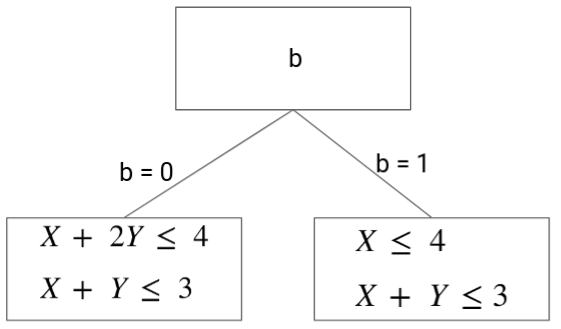
\includegraphics[scale=0.3]{Capitulos/Cap01_figs/branch-in-bound.png}
%     \caption{Arvore utilizada para realizar \textit{LP relaxation} e resolver individualmente os problemas de LP, ainda maximizando a equação \ref{eq:Cap01_MILP_Objective}.}
%     \label{fig:Cap01_TreeLP}
% \end{figure}
% Ao percorrer a arvore da figura \ref{fig:Cap01_TreeLP} resolvendo o LP comparando os resultados da equação \ref{eq:Cap01_MILP_Objective} e selecionando o melhor.
% \begin{itemize}
% \item
%   \textit{Web Service Description Language} \cite{wsdl:spec}: usada para
%     definir APIs que usam o protocolo SOAP. É uma linguagem baseada em XML.
%     Um exemplo de um arquivo WSDL é apresentado em \cref{anex:wsdl-example}.
% \item
%   \textit{OpenAPI} \cite{openapi:spec}: comumente usada para definir APIs que usam
%     o protocolo HTTP \cite{rfc2616}, informalmente chamadas de \textit{"Restful APIs"}
%     em referência ao conceito de REST definido em \cite{10.5555/932295}. É uma linguagem
%     baseada em YAML. Um exemplo de um arquivo OpenAPI é apresentado em \cref{anex:openapi-example}.
% \item
%   \textit{Protocol Buffers} \cite{googl:protobuf}: usada para definir APIs que usam
%     o protocolo gRPC \cite{googl:grpc}. O nome se refere tanto à IDL usada para a
%     especificação quanto para ao formato binário usado para transmitir as mensagens.
%     Um exemplo de um arquivo em Protocol Buffers é apresentado em \cref{anex:protobuf-example}.
% \end{itemize}

% Existem diversas vantagens em usar uma IDL, entre elas:

% \begin{enumerate}
% \item
%   A comunicação entre diferentes times (possivelmente em diferente organizações) que
%   precisam interagir via API é mais simples, já que todos os detalhes de interface
%   estão especificados em um formato padrão.
% \item
%   Pro esse motivo, é muito mais simples construir ferramentas de análise sobre a
%   especificação, como geradores de código, validadores, ferramentas de teste, etc.
% \end{enumerate}

\section{Algoritmo genético}

\cite{book:genetic_algo_data_structure}Algoritmos genéticos são algoritmos comumente utilizados para resolver problemas de otimização. 
Principalmente aqueles onde não podem ser equacionados, como certos problemas abstratos.
Estes não garantem uma solução ótima, mas com uma população suficientemente grande de genes e gerações pode-se reduzir as chances de erro ao menor possível.

Um algoritmo precisa ter essas características:
\begin{itemize}
\item
  Precisa possuir umas estrutura de dados que permite a fácil decodificação para uma combinação do resultado para o problema desejado, no caso do problema de empacotamento ela é convertida na posição dos objetos. Essas estruturas são chamadas de cromossomos e são comumente compostos por binários ou caracteres que são chamados de genes;
\item
  Criar a população inicial, onde o tamanho deve ser determinado pelos parâmetros;
\item
  Precisa de um método para avaliar a qualidade do cromossomo, como um sistema de score/fitness;
\item
  Um método de selecionar os cromossomos que originarão a população da próxima geração
\item
  Um método probabilístico de misturar conjuntos de genes da população vencedora. Pois estes conjuntos fazem parte de cromossomos que venceram diversas gerações, assim multiplicando bons conjuntos de genes através das gerações. Análogo ao que ocorre com a genética biológica. Este processo é chamado de cruzamento; 
\item
  Um método probabilístico de fazer pequenas alterações nos genes da próxima geração, assim gerando resultados próximos ao anterior, mas possivelmente melhores, assim é a caracterizado o processo de mutação.
\end{itemize}

\subsection{Estrutura de dados}
    No GA, a estrutura de dados que é utilizado para converter em informações do problema a ser resolvido é comumente chamado de cromossomo, que é um vetor de genes, onde estes são normalmente um bit, ou um caractere.

\begin{figure}[h]
    \centering
    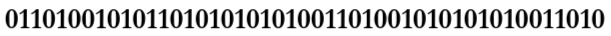
\includegraphics[scale=0.65]{Capitulos/Cap01_figs/genes_bit.png}
    \caption{Exemplo de uma gene onde os seus cromossomos são bits. Como a conversão desse gene se transforma em uma solução possível para o problema à ser resolvido, isso significa que para um gene de n bits, nos teremos $2^{n}$ soluções possíveis, fazendo a busca por força bruta ser impraticável para grandes valores de n.}
    \label{fig:Cap01_Genes_Bits_Example}
\end{figure}

\subsection{População de cromossomos}
É o conjunto de cromossomos, que são utilizados para possibilitar uma diversidade de genes desejada, que através da seleção, cruzamento e mutações apropriadamente calibradas, pode-se encontrar uma solução sub-ótima para o problema proposto.
\newline
Fatos a se ficar atento em uma população de genes é o risco da população começar a gerar respostas extremamente parecidas, fazendo o algoritmo ficar limitado em uma região de mínimo/máximo local. Fazendo-se necessária uma analise desse risco para a formulação dos algoritmos responsáveis pela geração seguinte.\newline

Outro fator que pode ser usado para acelerar a convergência para um bom resultado é a criação de uma população inicial bastante dispersa, aumentando as chances de diversos genes estarem próximos de pontos ótimos locais.\newline

\subsection{Avaliação}
Depois da decodificação de um cromossomo, se é feita uma função para quantificar a sua qualidade, assim permitindo comparação entre os cromossomos, consequentemente permitindo o processo de seleção, explicado na sub seção \ref{Cap_intro:sec_GA:sub_selection}.
\subsection{Seleção}\label{Cap_intro:sec_GA:sub_selection}
Pode-se desenvolver diversos algoritmos de seleção, onde um dos mais básicos e conhecidos é simplesmente escolher aleatoriamente dois cromossomos da população e o mais apto será copiado para compor a próxima geração, sendo este gene podendo ser selecionado múltiplas vezes, dessa forma a probabilidade de um conjunto de genes bons passar para a próxima geração aumenta.

\subsection{Cruzamento}
Devido ao fato dos cromossomos serem decodificados em dados para o problema desejado, dependendo como a estrutura dos genes é projetado, intervalos de genes de um cromossomo terão influencias no resultado de forma independente.\newline
Como exemplo: Pode-se pensar no caso do empacotamento, onde os cromossomos são divididos em intervalos iguais de genes, sendo que o primeiro intervalo representa a posição e rotação do primeiro objeto, o segundo intervalo representa o segundo objeto, seguindo essa logica até o fim.\newline
Ao termos genes compostos dessa forma, a população de genes pode possuir valores onde os cromossomos para objeto 2 do Cromossomo 1, melhoraria o Cromossomo 2. Fazendo-se desejável a formação de um novo cromossomo com os genes do segundo com os genes do objeto 2 do Cromossomo 1. Assim mostrando a relevância de cruzamento para o algoritmo genético.\newline
\begin{figure}[h]
    \centering
    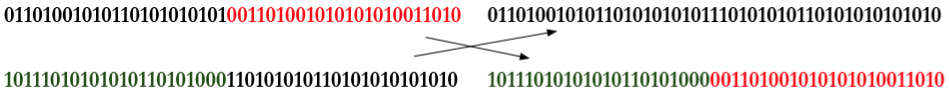
\includegraphics[scale=0.45]{Capitulos/Cap01_figs/cruzamento_pivot.png}
    \caption{Exemplo de um cruzamento de dois genes, onde ocorre a troca por entre as regiões delimitadas apenas por um pivô.}
    \label{fig:Cap01_cruzamento_pivot_Example}
\end{figure}
\newline
Apesar da figura \ref{fig:Cap01_cruzamento_pivot_Example} ser um cruzamento com o intervalo dos genes a serem cruzados delimitado por apenas um pivô, ou seja do pivô até o ultimo gene serão trocados. Pode-se fazer o cruzamento de outras formas, como num problema de empacotamento, é provavelmente mais interessante propor cruzamento com dois pivôs, onde um determina o primeiro e o outro o ultimo cromossomo trocado. Estes pivôs podem ser determinados de forma a tentar trocar os genes de objetos por inteiro ou parciais. Assim os melhores genes para um determinado objeto serão multiplicados com o passar das gerações.

\subsection{Mutação}
Com apenas os processos de seleção e cruzamento, o GA muito provavelmente ficaria preso em um ótimo local e sua população se tornaria muito parecida extremamente rápido. Dessa forma se faz necessário alterar os valores dos genes dos cromossomos de forma aleatória, mas não grosseira de forma que o cromossomo sofra poucas alterações de cada vez, assim garantindo uma diversidade a população e aumentando as probabilidades de se encontrar um valor de cromossomo melhor.

\subsection{Parâmetros}
 A escolha dos parâmetros é muito importante para um algoritmo genético, pois eles possuem grande influencia em como a população de genes de transforma ao passar da gerações, onde eles são definidos na lista abaixo da apostila \cite{algo_genetics_principios}:\newline
\begin{itemize}
\item
    Tamanho da População: Numero de espaço de busca sendo considerados em paralelo a cada ciclo
\item
    Taxa de \textit{crossover}: probabilidade(p\textunderscript{c}) de um individuo ser recombinado com outro(Cruzamento).
\item
    Taxa de mutação: probabilidade(p\textunderscript{m}) do conteúdo de uma posição/gene do cromossomo ser alterado.
\item
    Numero de gerações: Total de ciclos de uma evolução de um GA.
\item
    Total de indivíduos: total de tentativas em um experimento(tamanho da população x numero de gerações).
\end{itemize}

Sendo os dois últimos parâmetros são geralmente usados como critério de parada.

\section{Problemas}\label{cap:introducao:sec:problema}
Um dos problemas que serão propostos é inspirado em \textit{knolling}, que é uma tendência de estilo fotográfico onde se organizam objetos em uma figura de forma comumente retangular, mas ela pode ter múltiplas formas como no exemplo da figura \ref{fig:Cap01_Knolling_Photography_43}.
\begin{figure}[H]
    \centering
    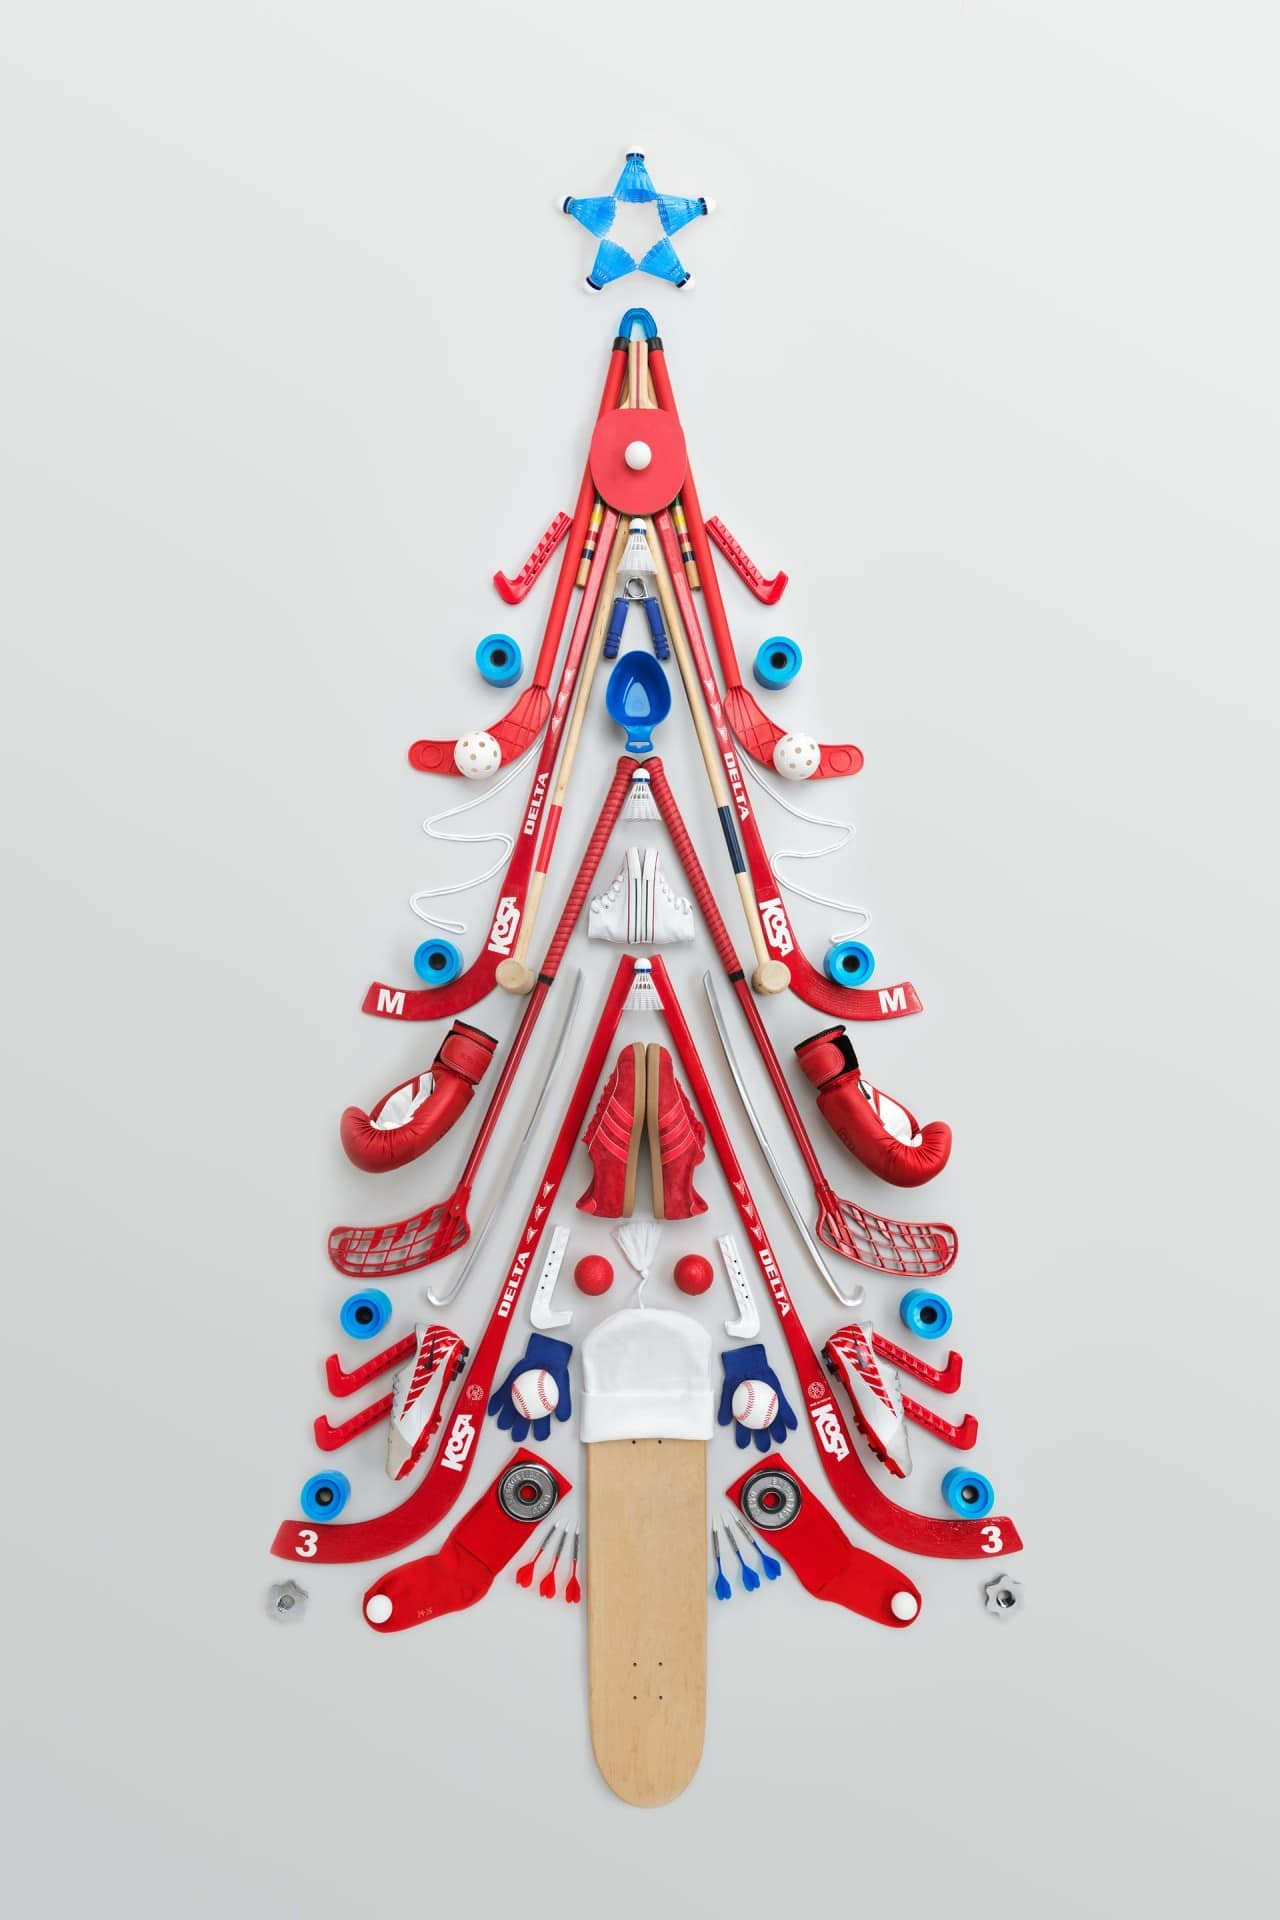
\includegraphics[scale=0.2]{Capitulos/Cap01_figs/Knolling-Photography-43.jpg}
    \caption{Exemplo de uma fotografia no estilo \textit{knolling} extraída de um site\cite{knolling:blog}. Onde se organiza os objetos formando uma figura alternativa.}
    \label{fig:Cap01_Knolling_Photography_43}
\end{figure}
Dessa forma serão proposto dois problemas à serem resolvidos por algoritmo genético:
\begin{enumerate}
\item
  Empacotar objetos tridimensionais num plano bidimensional de forma a obter um retângulo de menor área.
\item
  Empacotar objetos tridimensionais em um plano bidimensional dentro de uma região delimitada por uma forma geométrica, como está exemplificada na figura \ref{fig:Cap01_Knolling_Photography_43}. 
\end{enumerate}
% \begin{enumerate}
% \item
%   Como toda a parte dos modelos são geradas, servidor ou cliente, há uma significativa
%   redução no volume de linhas de código-fonte do sistema, reduzindo a possibilidade
%   de defeitos \cite{5010260} e facilitando o entendimento do projeto por novos
%   desenvolvedores.
% \item
%   Como o código é gerado a partir da especificação, sabemos que a implementação
%   vai estar de acordo com a interface especificada, permitindo que o programador
%   foque em implementar a lógica de cada operação, otimizando o uso do tempo. No
%   caso de consumidores, eles poupam o trabalho de ter que implementar um código
%   de integração com a API, que pode conter erros e ser difícil de manter,
%   principalmente com relação a mudanças e adições na API.
% \item
%   O código gerado abstrai toda a camada de comunicação e rede, tanto do servidor
%   quanto do cliente, facilitando o entendimento do código que o programador precisa
%   implementar.
% \end{enumerate}

% Existem diversos exemplos de geradores de APIs, alguns são \cite{openapi:gen} e
% \cite{googl:protobuf}.

% \section{ORMs}

% Da mesma forma que IDLs e geradores tentam facilitar o desenvolvimento da
% \textit{interface} de uma API, ORMs tentam facilitar a integração do código da
% API com o banco de dados usado (seja ele SQL ou NoSQL). Elas são bibliotecas que
% abstraem a execução de operações no banco de dados em uma interface amigável para
% a linguagem de programação usada. Por esse motivo, ORM é específica para a linguagem
% de programação em que ela foi implementada, e normalmente também é específica para
% um banco ou conjunto de bancos.

% ORMs normalmente funcionam via anotações e interfaces que o programador precisa
% adicionar ou implementar no código-fonte dos modelos. Essas anotações servem para,
% por exemplo, mapear o modelo a uma tabela, um campo a uma coluna, ou uma relação
% com outro modelo (1-1, 1-muitos ou muitos-muitos).

% Um exemplo em Python usando a ORM \texttt{sqlalchemy} é \cref{lst:sqlalchemy-example}.

% \begin{listing}[ht]
% \begin{minted}{python}
% from sqlalchemy import Column, DateTime, String, Integer, ForeignKey, func
% from sqlalchemy.orm import relationship, backref
% from sqlalchemy.ext.declarative import declarative_base


% Base = declarative_base()


% class Department(Base):
%     __tablename__ = 'department'
%     id = Column(Integer, primary_key=True)
%     name = Column(String)


% class Employee(Base):
%     __tablename__ = 'employee'
%     id = Column(Integer, primary_key=True)
%     name = Column(String)
%     # Use default=func.now() to set the default hiring time
%     # of an Employee to be the current time when an
%     # Employee record was created
%     hired_on = Column(DateTime, default=func.now())
%     department_id = Column(Integer, ForeignKey('department.id'))
%     # Use cascade='delete,all' to propagate the deletion of a Department
%     # onto its Employees
%     department = relationship(
%         Department,
%         backref=backref('employees',
%                          uselist=True,
%                          cascade='delete,all'))

% \end{minted}
% \caption{Exemplo de código usando \texttt{sqlalchemy}}
% \label{lst:sqlalchemy-example}
% \end{listing}

% ORMs são populares pois simplificam o trabalho do desenvolvedor ao automatizar muitas
% operações que são comumente realizadas no banco, e por prover uma DSL caso seja
% necessário fazer algo mais complexo. Dependendo da linguagem, essas funcionalidades
% podem ser validadas em tempo de compilação, previnindo defeitos.

% \section{Problema}

% Apesar de serem ferramentas muito populares, geradores de APIs e ORMs não integram
% bem. O primeiro costuma focar na \textit{interface de comunicação}, não prestando
% atenção a detalhes de implementação. Além disso, dado o grande número de ORMs
% presente para cada linguagem, e também as diversas formas de se gerar a interface
% de comunicação, geradores convencionais não conseguiriam adicionar suporte para
% todas as combinações possíveis.

% Outro problema em como os geradores são implementados hoje é que eles possuem
% suporte limitado a extensões externas ao código-fonte. Dependendo do gerador
% utilizado, é necessário implementar um \textit{novo gerador}, o que gera um grande
% custo operacional. Alguns exemplos de modificações possíveis:

% \begin{itemize}
% \item
%   Geração automática de testes para as operações \cite{9159071}.
% \item
%   Validação automática de propriedades das mensagens \cite{envoy:protoc-gen-validate}.
% \item
%   Integração com ORMs ou outras bibliotecas.
% \end{itemize}

% Devido a esses problemas, muitas organizações deixam de usar essas ferramentas e os
% programadores precisam implementar manualmente códigos que poderiam ser gerados.
% Isso aumenta a chance de erros ocorrerem durante a implementação, e o resultado divergir
% da especificação. Além disso, diminui a eficiência do time, pois há mais tarefas a
% serem realizadas.

% Avaliando as tarefas realizadas pelo time de engenharia de uma organização durante o
% ano de 2020, foi possível identificar que pelos menos 30\% das tarefas realizadas
% eram relacionadas a implementação de modelos, integração com ORMs e com a camada
% de comunicação da API. Além disso, dentro desses 30\%, ocorreram diversas vezes tarefas
% extras relacionadas com ajustes da implementação para que essa seguisse a especificação.

% Na tentativa de solucionar esse problema, esse trabalho propõe um novo modelo de
% gerador de APIs, que pode ser extendido para suportar qualquer linguagem ou funcionalidade
% nova sem a necessidade de modificar o código-fonte.

% Esse trabalho é estruturado como se segue. \cref{cap:past-works} faz uma análise
% de trabalhos anteriores. \cref{cap:proposal} apresenta, de forma detalhada, o que
% foi construído e a metodologia de análise.


% \chapter{Trabalhos Anteriores}\label{cap:past-works}
\chapter{Ferramentas a serem utilizadas}\label{cap:tools}
% TODO: maybe talk about LLVM here?

A lista de ferramentas a serem utilizadas está logo abaixo:

\begin{itemize}
    \item \textit{FreeCad 0.19} para o uso e apresentação das peças tridimensionais, pois ele possui um ótima integração com \textit{Python}, assim permitindo uma implementação visual do algoritmo de empacotamento.
    \item \textit{Python} pela possibilidade de integração com o \textit{FreeCad} e de usar código feito em \textit{C++}.
    \item \textit{C++} para possibilitar um algoritmo genetico de mais baixo nivel, utilização do CGAL para a utilização de algoritmos geométricos e Boost para desenvolver um modulo para \textit{Python} e a classe \textit{dynamic\_bitset} para ser usado para os genes.
\end{itemize}

\section{FreeCad}\label{cap:tools:sec:freecad}

\cite{FreeCad} É um \textit{software} de modelagem \textit{open source} com uma \textit{API} para \textit{Python}, permitindo assim desenvolver códigos para alterar suas cenas tridimensionais ou minerar os dados da mesma.

\subsection{Integração com \textit{Python}}
\begin{figure}[H]
    \centering
    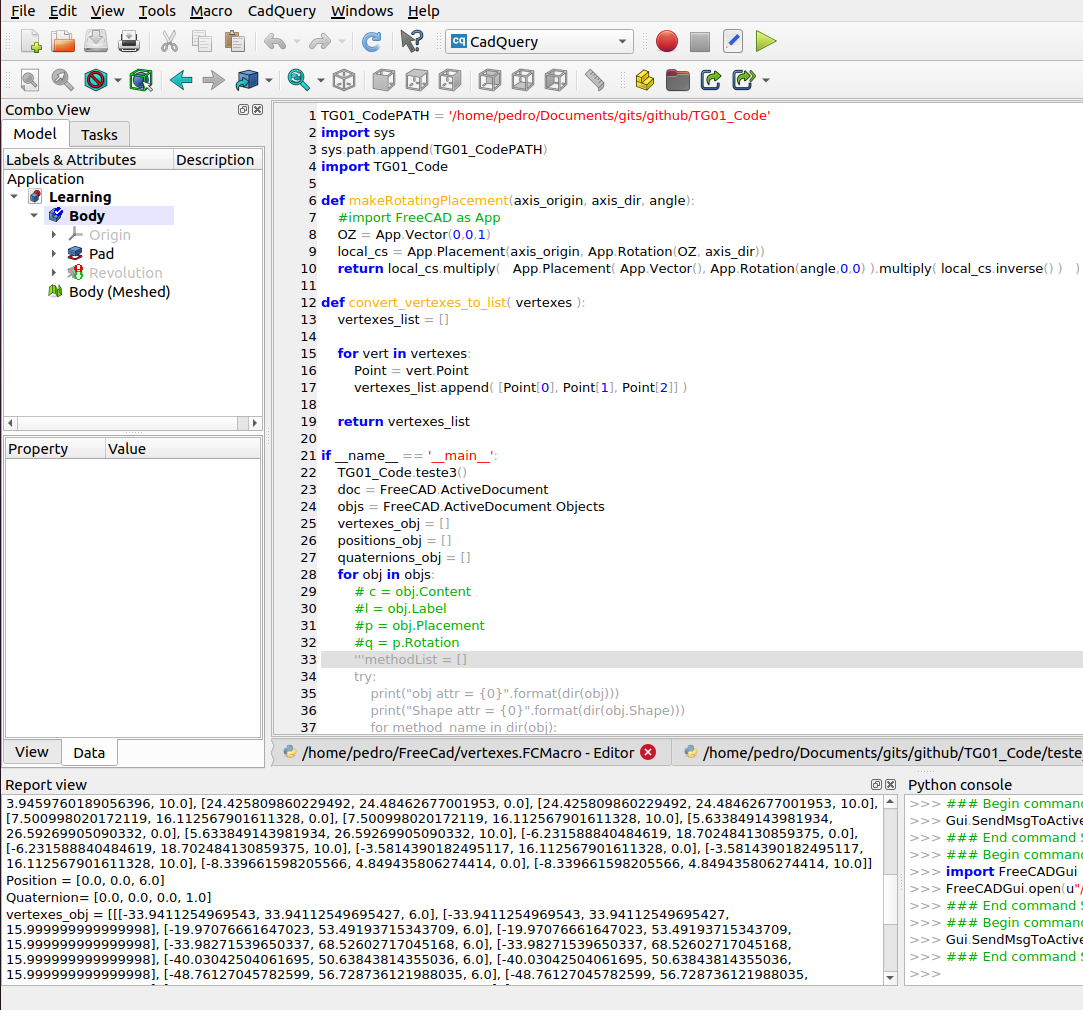
\includegraphics[scale=0.3]{Capitulos/Cap02_figs/FreeCad_Python.png}
    \caption{Exemplo da execução de um código de \textit{Python} no \textit{FreeCad}, onde se pega os vértices, posição e a rotação por \textit{quaternion} dos objetos da cena}
    \label{fig:Cap02_FreeCad_Python_01}
\end{figure}

\textit{FreeCad}, ao poder executar um \textit{script} que interage com os objetos da cena, permitindo acesso aos atributos listados abaixo:
\begin{itemize}
    \item \textit{Placement}: Objeto \textit{Python} que possui os valores associados a posição e rotação do modelo 3D.
    \begin{itemize}
        \item \textit{Base}: Objeto \textit{Python} que possui  posição (x, y, z).
        \item \textit{Rotation}: Objeto \textit{Python} que possui os valores da rotação do objeto, podendo adquirir a rotação por um Eixo, ou os valores em \textit{quaternion}.
    \end{itemize}
    \item \textit{Shape}: Atributo do objeto que possui informações da forma do modelo tridimensional, como os vértices e arestas.
    \begin{itemize}
        \item \textit{Vertexes}: É a lista dos vértices, que possuem o atributo \textit{Point} que é o valor das posições do vértice no eixo XYZ.
        \item \textit{Edges}: É a lista das arestas da forma tridimensional. 
    \end{itemize}
\end{itemize}

Assim garantindo que os dados dos objetos seja de fácil obtenção.

\section{\textit{C++}}
O \textit{C++} sera a ferramenta principal do trabalho, pois o código em \textit{C++} será o responsável por receber os dados brutos dos objetos da cena do \textit{FreeCad} como vértices, arestas, posições e rotação. Retornando as informações necessárias para que o \textit{FreeCad} reposicione os seus elementos na posição e rotação desejada. \newline
Dessa forma o código em \textit{C++} será responsável por:

\begin{enumerate}
    \item Pré-processamento: Os dados de posição e vértices de cada peça obtidos do \textit{FreeCad} vão ser armazenados por estruturas de dados do \textit{CGAL}\cite{cgal:complete_manual}, assim sendo projetados no plano XY, em seguida será determinado a forma poligonal a ser obtida usando o algoritmo do fecho convexo\cite{cgal:convex_hull}.
    \item Empacotamento: Usando um algoritmo genético para se determinar as posições e rotações dos polígonos, no qual seja encontrado uma solução para o problema proposto, podendo ser o de empacotar na menor areá retangular ou dentro de uma forma geométrica assim como \textit{knolling}.
    \item Pós-processamento: Uma forma de passar determinar a translação e rotação a ser realizada nas peças do \textit{FreeCad} para mostrar o empacotamento na cena.
\end{enumerate}

\subsection{\textit{CGAL}}

\cite{cgal:software} É uma sigla para \textit{Computational Geometry Algorithms Library}, em português significa Livraria de algoritmos de geometria computacional.\newline
\cite{cgal:complete_manual}\textit{CGAL} é um projeto de \textit{software} que provê algoritmos eficientes e confiáveis na forma de uma biblioteca de \textit{C++}.\textit{CGAL} é usado em varias áreas onde é necessário computações geométricas, como sistemas de informação geográfica, biologia molecular, imagens medica, computação gráfica e robótica.\newline

A biblioteca oferece estruturas de dados e algoritmos como triangulação, diagramas de Voronoy, operações boolianas com polígonos e poliedros, processamento de conjuntos de pontos, arranjos de curvas e superfícies, processamento de geometria, formas alfas, algoritmos de fecho convexo, entre outras funcionalidades. \newline

\cite{cgal:convex_hull}A função de fecho convexo tem sua funcionalidade que será utilizar os pontos projetados de cada objeto 3D para formar o seu respectivo polígono no plano XY, dessa forma pode-se determinar sobreposições, realizar translação e rotações dos polígonos, assim permitindo o uso do algoritmo genético para a solução do problema proposto na seção \ref{cap:introducao:sec:problema}.

\begin{figure}[H]
    \centering
    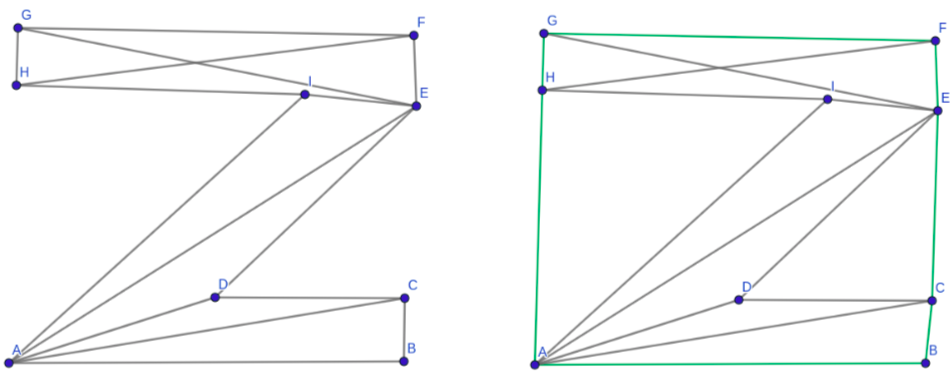
\includegraphics[scale=0.4]{Capitulos/Cap02_figs/CGAL_Convex_EX.png}
    \caption{Exemplo de um objeto projetado com suas arestas no plano XY, com os seus vértices sendo processados pela função do fecho convexo no lado direito, pode-se ver que nesse exemplo ocorre um consumo maior de espaço do que o necessário, devido ao fato do polígono a ser formado ter que ser convexo.}
    \label{fig:Cap02_CGAL_Convex_EX}
\end{figure}

Como para o problema de empacotamento, nos não queremos que ocorra sobreposição dos polígonos, logo será usado funções para se determinar intersecções entre os polígonos, assim influenciando na seleção do GA.

\subsection{\textit{Boost}}
\cite{boost:software} \textit{Boost} provê fontes de bibliotecas portáveis de \textit{C++} revisadas por pares.\newline
Enfatiza que as bibliotecas vão funcionar bem com a \textit{Standard Library} do \textit{C++}. As bibliotecas do \textit{Boost} são pensadas para terem um uso abrangente, e usabilidade para diversos tipos de aplicações. A licença do \textit{Boost} encoraja o uso de suas bibliotecas para todos os usuários com o mínimo de restrições.

\cite{boost:Python} A biblioteca \textit{Boost Python} é um \textit{framework} para fazer a interface entre \textit{Python} e \textit{C++}. O que permite uma forma simples e rápida de expor as classes, objetos e funções do \textit{C++} para o \textit{Python}, e vice-versa, sem a necessidade de ferramentas além do compilador de \textit{C++}. Ela é formulada para integrar \textit{C++} de forma não intrusiva, de tal modo que não seja necessário fazer qualquer alteração do código de \textit{C++}, fazendo \textit{Boost.Python} ideal para expor bibliotecas de terceiros ao \textit{Python}. A biblioteca usa técnicas avançadas de meta-programação para simplificar a sua sintaxe aos usuários, de forma que integrar o código toma uma forma de IDL declarativa.\newline
Assim será usada para integrar o código em \textit{Python} com o de \textit{C++}.

\cite{boost:dynamic_bitset}A classe \textit{dynamic\_bitset} representa um conjunto de bits. Este provê o acesso ao bit individualmente pelo operador [ ] e provê operadores de bits que só podem ser aplicados à inteiros nativos de \textit{C++}, como o operador \&. O número de bits pode ser especificado durante a execução como parâmetro do construtor do \textit{dynamic\_bitset}, o que o torna uma opção mais atrativa que o \textit{bitset} da \textit{Standard Library}, que tem o seu tamanho definido na compilação. Assim fazendo uma ótima estrutura de dados para os genes do GA.

% \cite{openapi:gen} apresenta uma vasta gama de geradores baseados na IDL OpenAPI. Até
% a presente data, apresenta 66 geradores de clientes para 33 linguagens e 41 geradores
% de servidores para 16 linguagens. Esse é o principal programa utilizado para gerar
% código em projetos que usam OpenAPI para especificação de suas APIs.

% Analisando o código-fonte e documentação do projeto, chegamos às seguintes conclusões:

% \begin{itemize}
% \item
%   Os geradores funcionam com base em um modelo genérico baseado em OpenAPI. O processo
%   de geração ocorre da seguinte maneira:

%   \begin{enumerate}
%   \item
%     O programa lê a especificação OpenAPI e a transforma no modelo genérico.
%   \item
%     A classe do gerador modifica esse modelo da forma que precisar, possivelmente
%     adicionando propriedades específicas para ele.
%   \item
%     O programa envia o modelo final para um motor de \textit{templates}, que
%     carrega os templates do gerador específico e os renderiza. O resultado dessa
%     etapa é o código final.
%   \end{enumerate}

%   Esse fato pode acabar por limitar a expressividade do gerador, pois o modelo
%   OpenAPI não é capaz de expressar, de forma simples, todos os detalhes envolvidos
%   em uma linguagem de programação.
% \item
%   Apesar de ser possível criar um novo gerador customizado, por exemplo, para uma
%   linguagem que o projeto não suporte, sem a necessidade de modificar o programa
%   em si, os geradores são estruturas monolíticas. Não é possível implementar uma
%   funcionalidade nova, e.g. um novo processo de validação, que possa ser usado por
%   todos os geradores. Isso limita significativamente a extensibilidade do projeto,
%   além de aumentar a carga operacional nessas situações.
% \end{itemize}

% \cite{googl:protobuf} é o compilador de Protocol Buffers. Ele apresenta uma estrutura
% bastante interessante em questão de extensibilidade: o sistema de \textit{plugins}.
% Um \textit{plugin} é um programa que recebe uma mensagem \texttt{CodeGeneratorRequest}
% como entrada e escreve na saída uma mensagem \texttt{CodeGeneratorResponse}. As
% definições dessas duas mensagens são apresentadas em \cref{lst:code-gen-req} e
% \cref{lst:code-gen-res}, respectivamente.

% \begin{listing}[ht]
% \caption{Especificação de \texttt{CodeGeneratorRequest}}
% \label{lst:code-gen-req}
% \begin{minted}{protobuf}
% message CodeGeneratorRequest {
%   repeated string file_to_generate = 1;

%   optional string parameter = 2;

%   repeated FileDescriptorProto proto_file = 15;

%   optional Version compiler_version = 3;
% }
% \end{minted}
% \end{listing}

% \begin{listing}[ht]
% \caption{Especificação de \texttt{CodeGeneratorResponse}}
% \label{lst:code-gen-res}
% \begin{minted}{protobuf}
% message CodeGeneratorResponse {
%   optional string error = 1;

%   message File {
%     optional string name = 1;

%     optional string insertion_point = 2;

%     optional string content = 15;
%   }

%   repeated File file = 15;
% }
% \end{minted}
% \end{listing}

% Esse sistema é interessante por dois fatores:

% \begin{itemize}
% \item
%   É muito simples adicionar suporte a uma nova linguagem, precisamos apenas
%   implementar um \textit{plugin}. Ponto em comum com o trabalho anterior.
% \item
%   Usando o campo \texttt{file.insertion\_point}, é possível injetar conteúdo
%   de um gerador em outro. O segundo gerador pode adicionar esses pontos no
%   arquivo gerado por ele, permitindo que outros geradores modifiquem o resultado
%   final.

%   Isso soluciona, em parte, o problema de adicionar novas funcionalidades em
%   um gerador presente em \cite{openapi:gen}. Dois problemas ainda persistem:

%   \begin{enumerate}
%   \item
%     Estamos limitados aos pontos de inserção disponibilizados pelo gerador, o
%     que pode variar de uma linguagem para outra. O quão grave é esse problema
%     depende do que se quer fazer com o \textit{plugin} e qual é a linguagem objeto.
%   \item
%     O sistema trabalha em termos de texto (campo \texttt{file.content}). Isso
%     limita o quão genérico nossa funcionalidade pode ser, e.g. um \textit{plugin} de
%     validação poderia ser genérico caso o resultado fosse mais estruturado.

%     Um exemplo de plugin que poderia ser genérico é \cite{envoy:protoc-gen-validate},
%     que provê uma extensão para diversas validações. Hoje, ela é limitada para
%     as linguagens Go, C++ e Java. Caso o resultado fosse mais estruturado, seria
%     possível implementar tal funcionalidade de forma genérica para uma grande
%     quantidade de linguagens.
%   \end{enumerate}
% \end{itemize}

% \cite{9159071} se propõe a resolver um problema diferente dos trabalhos anteriores:
% ele gera testes baseado em \textit{Property Based Testing} \cite{10.1145/351240.351266}
% a partir de especificações OpenAPI que validam que as respostas da API seguem as
% propriedades e formatos especificados. O programa é capaz de gerar esses testes
% sem a necessidade de nenhuma extensão a especificação.

% \cite{sferruzza:hal-01868498} propõe extensões e um gerador para OpenAPI que é
% capaz de modelar como uma operação é implementada. O trabalho cria o conceito de
% \textit{componentes atômicos e compostos}: componentes atômicos recebem parâmetros
% e podem gerar novos valores e componentes compostos fazem a composição de diversos
% componentes para definir uma dada lógica. O programa então é capaz de validar que
% as definições e uso dos componentes são válidas, tanto em questão de todas as
% variáveis estarem disponíveis quanto que os tipos estão corretos. O gerador é capaz
% de gerar código que define esses componentes.

% Por fim, \cite{r2c:semgrep} é uma ferramenta de análise estática que suporta uma
% quantidade impressionante de linguagens. O diferencial dessa ferramenta é que
% o usuário pode criar novas regras de análise utilizando uma DSL implementada sobre
% YAML, permitindo com que a mesma regra seja aplicada em diversas linguagens. Isso
% é possível pois todas as linguagens que ela suporta são convertidas para
% \textit{uma mesma linguagem intermediária} antes das regras serem aplicadas. Essa
% funcionalidade é similar a situação em que queremos implementar uma funcionalidade
% no nosso gerador de forma independente da linguagem objeto.


\chapter{ Metodologia }\label{cap:proposal}
\section{Processamento da cena do \textit{Freecad}}
Para se iniciar a resolver o problema, é necessário processar os objetos da cena do \textit{FreeCad}, assim permitindo a mineração dos dados destes objetos.

Para o problema de encontrar o empacotar em um retângulo de menor área, referido na seção \ref{cap:introducao:sec:problema}, deve-se seguir a logica abaixo:
\begin{enumerate}
    \item Minimização de altura: Rotaciona os objetos para que as suas faces estejam no plano Z = 0, e que a altura do objeto seja minimizada;
    \item Posição inicial: Reposiciona os objetos em uma posição inicial onde os seus vértices nas coordenadas XY, tenham os seus valores máximos no zero, o motivo, se dá ao fato que o algoritmo genético irá somar a translação destes objetos;
    \item Coleta dos vértices: Será coletado os vértices de cada objeto da cena, e estes serão enviados para o código de \textit{C++}, este irá pre-processar os dados dos vértices, processar o \textit{GA} enquanto salva a performance;
    \item : Será coletado os vértices de cada objeto da cena, e estes serão enviados para o código do \textit{GA}, este irá pre-processar os dados dos vértices, processar o \textit{GA} enquanto salva a performance.
\end{enumerate}

Para o caso de \textit{Knolling}, deve-se adicionar os seguintes passos antes de passar os dados para o código do \textit{C++}:
\begin{enumerate}
    \item Posicionamento da bandeja: Reposiciona a bandeja para que os vértices de menor valor X e Y estejam posicionados no zero;
    \item Coleta dos vértices da bandeja: Se coleta os vértices da bandeja para se usar no \textit{GA}.
\end{enumerate}

\subsection{Minimização da altura}
Para se alocar os objetos em uma bandeja de impressão 3D, se é interessante limitar a altura desses objetos.\newline
Com o intuito de minimizar a altura dos objetos foi feito uma função, com a logica abaixo: 
\begin{enumerate}
    \item Realiza um \textit{loop} por todos os objetos da cena do tipo ``<class `PartDesign.Body'>" e que não possuam o nome "Board Body", pois este está reservado para a bandeja;
    \begin{enumerate}
        \item Realiza um \textit{loop} por todas as faces
        \begin{enumerate}
            \item Onde se verifica a distância de todos os vértices;
            \item Caso essa distância seja menor que a menor altura registrada, esta face será a nova melhor;
        \end{enumerate}
        \item Ao se determinar a melhor face, se determina o vetor normal dessa face;
        \item Partindo desse valor é possível determinar o eixo de rotação e o angulo, assim se determinando o "\textit{spin}";
        \item Ao rotacionar o objeto, se é necessário se determinar a altura do vértice mais baixo, este provavelmente será qualquer vértice da face encontrada, mas foi decidido verificar todos, pois esse pre-processamento não é significativo para o tempo de execução;
        \item Usa a altura do vértice de menor valor em Z para desloca-lo para o plano Z = 0, assim demostrado na figura \ref{fig:Cap03_FreeCad_Rotation}.
    \end{enumerate}
\end{enumerate}

A função "\textit{Rotate2ShorterstHeight}" do \cite{code:FreeCad_Miner}, pode ser encontrada abaixo:

\begin{lstlisting}[language=Python, breaklines, caption = \textit{Rotate2ShorterstHeight}, captionpos=b]
def Rotate2ShorterstHeight( objs ):
    for obj in objs:
        if 'Shape' in dir(obj):
            if str(type(obj)) == "<class 'PartDesign.Body'>" and obj.Label != "Board Body":
                s = obj.Shape
                p = obj.Placement
                b = p.Base
                faces = s.Faces
                size_list = len(faces)
                best_face = -1
                smallest_height = 9999999

                #Look through object faces, looking for the 
                #one which on the bottom would gives us the shortest height
                for i in range( size_list ):
                    height = -1
                    for j in range( size_list ):
                        if i == j:
                            continue
                        for vertex in faces[j].Vertexes:
                            distance = faces[i].distToShape( vertex )[0]
                            if height < distance:
                                height = distance
                    print( "height = ", height )
                    if height < smallest_height:
                        smallest_height = height
                        best_face = i

                #Find Axis and angle to rotate
                uv = faces[ best_face ].Surface.parameter(faces[ best_face ].CenterOfMass)
                faceNormalInCOM = faces[ best_face ].normalAt(uv[0], uv[1])
                angle = acos( -faceNormalInCOM[2] )*180/(pi)

                # Make rotaion, so that face is on the bottom, and orthogonal to XY
                spin = makeRotatingPlacement(App.Vector(b[0], b[1], b[2]), App.Vector(-faceNormalInCOM[1], faceNormalInCOM[0], 0), angle)
                obj.Placement = spin.multiply(obj.Placement)

                #After rotation, sets find lowest high and sets it on zero
                s = obj.Shape
                p = obj.Placement
                b = p.Base
                r = p.Rotation
                lowest_height = 9999999
                for vertex in s.Vertexes:
                    Point = vertex.Point
                    if lowest_height > Point[2]:
                        lowest_height = Point[2]

                obj.Placement = App.Placement(App.Vector(b[0], b[1], b[2] - lowest_height), r)
\end{lstlisting}

\begin{figure}[H]
    \centering
    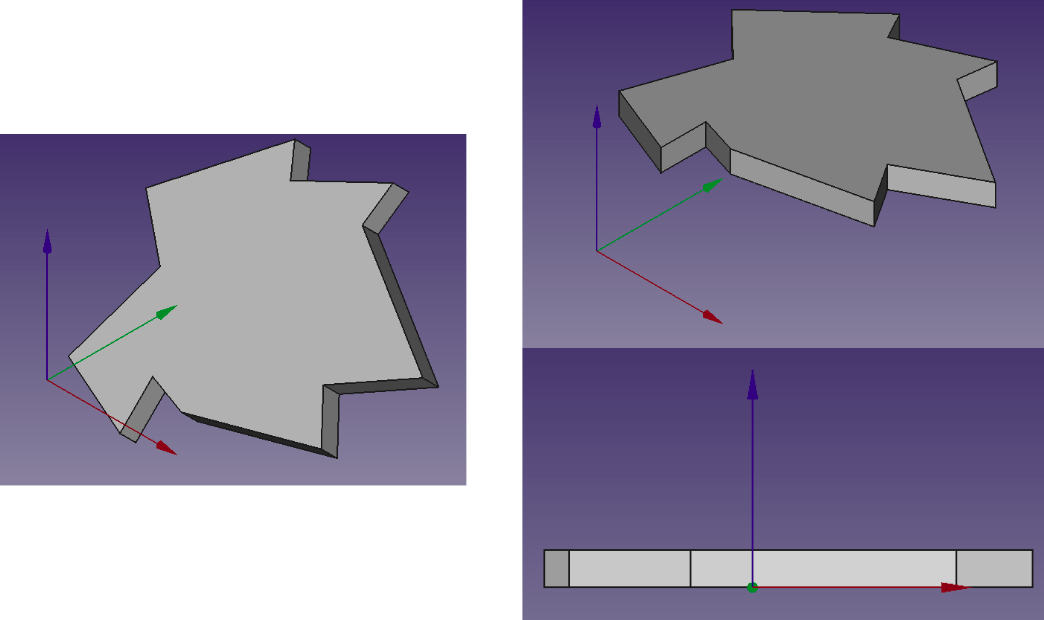
\includegraphics[scale=0.4]{Capitulos/Cap03_figs/Rotation_Face.png}
    \caption{Figura para se usar como exemplo da rotação, onde a imagem do lado esquerdo está é antes de se rotacionar, ou seja a altura não esta minimizada. Enquanto as do lado direito estão em diferentes perspectivas, para mostrar que passaram pela rotação}
    \label{fig:Cap03_FreeCad_Rotation}
\end{figure}
\subsection{Posição inicial}\label{cap:methods:initial_pos}

Após rotacionar os objetos, eles serão transladados em uma posição inicial, pois o algoritmos genético irá realizar uma translação dos objetos. Onde o vetor de translação, serão positivos em todos os eixos, logo se é interessante ter todos os vértices possuírem valores negativos em suas coordenadas.

\begin{enumerate}
    \item Realiza um \textit{loop} por todos os objetos da cena do tipo ``<class `PartDesign.Body'>" e que não possuam o nome "Board Body", pois este está reservado para a bandeja;
    \begin{enumerate}
        \item Realiza um \textit{loop} por todos os vértices;
        \begin{enumerate}
            \item Onde se verifica a coordenada dos vértices;
            \item Anotando a coordenada do maior valor de X e Y;
        \end{enumerate}
        \item Ao se determinar os maiores valores de X e Y, o objeto será transladado onde esses vértices estarão na posição zero de suas respectivas coordenadas, vide figura \ref{fig:Cap03_FreeCad_Initial_Position}.
    \end{enumerate}
\end{enumerate}

A função "\textit{Initial\_Position}" do \cite{code:FreeCad_Miner}, pode ser encontrada abaixo:

\begin{lstlisting}[language=Python, breaklines, caption = \textit{Initial\_Position}, captionpos=b]
def Initial_Position( objs ):
    #Go through every object
    for obj in objs:
        if 'Shape' in dir(obj):
            if str(type(obj)) == "<class 'PartDesign.Body'>" and obj.Label != "Board Body":
                s = obj.Shape
                p = obj.Placement
                b = p.Base
                r = p.Rotation
                #Set a realy low coordinate value on the highest at first, so it will switch for sure
                highest_x = -9999999
                highest_y = -9999999
                #Go through vetexes, looking for the highest values    
                for vertex in s.Vertexes:
                    Point = vertex.Point
                    if highest_x < Point[0]:
                        highest_x = Point[0]
                    if highest_y < Point[1]:
                        highest_y = Point[1]
                #Set new positions for object 'obj'
                obj.Placement = App.Placement(App.Vector( b[0]-highest_x, b[1]-highest_y, b[2], r) )
\end{lstlisting}

\begin{figure}[H]
    \centering
    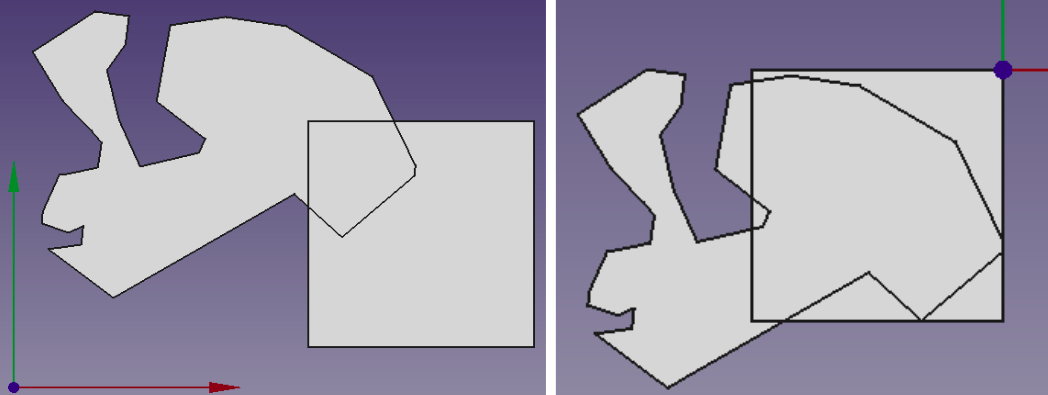
\includegraphics[scale=0.4]{Capitulos/Cap03_figs/Initial_Position.png}
    \caption{Ilustrando o resultado da função ao se rodar ela pelo \textit{FreeCad}, com a perspectiva, sendo vista de cima, para melhor mostrar o resultado da translação. Onde a imagem do lado esquerdo é a imagem da cena antes do código, e o da direita é a cena depois}
    \label{fig:Cap03_FreeCad_Initial_Position}
\end{figure}

\subsection{Coleta dos vértices}

Esse processo é necessário, devido a necessidade de se conhecer as formas dos objetos para ser possível empacota-los. Então os objetos serão processados para se coletar as coordenadas dos vértices, usando a logica abaixo:

\begin{enumerate}
    \item Realiza um \textit{loop} por todos os objetos da cena;
    \begin{enumerate}
        \item Armazena o valor da \textit{Base} dos objetos do cena, onde este é o ``centro" do objeto, não necessariamente da forma geométrica, e sim do objeto de computador. Mas devido ao fato de se reposicionar os objetos em \ref{cap:methods:initial_pos}, esse valor não é mais necessário; 
        \item Realiza um \textit{loop} por todos os vértices;
        \begin{enumerate}
            \item Anota as coordenadas X, Y e Z dos mesmos;
        \end{enumerate}
        \item Ao finalizar o processo, todas as posições e os valores das posições dos vértices estarão alocados em um lista do \textit{python}, pronto para se passar para o \textit{GA}.
    \end{enumerate}
\end{enumerate}

A função "\textit{getPositionsValues}" do \textit{script} \cite{code:FreeCad_Miner} será a responsável por esse processo:

\begin{lstlisting}[language=Python, breaklines, caption = \textit{getPositionsValues}, captionpos=b]
def getPositionsValues(objs):
    vertexesAll = []
    positions = []
    CadData = []
    for obj in objs:
        if 'Shape' in dir(obj):
            if str(type(obj)) == "<class 'PartDesign.Body'>" and obj.Label != "Board Body":
                p = obj.Placement
                b = p.Base
                #Stores position
                positions.append( [ b[ 0 ], b[ 1 ], b[ 2 ] ] )
                vertexes = obj.Shape.Vertexes
                #Object's Vertexes
                vertexes_list = []
                for vert in vertexes:
                    vertexes_list.append([vert.Point[0], vert.Point[1], vert.Point[2]])
                    
                #Vertexes for all objects
                vertexesAll.append(vertexes_list)
    return [ positions, vertexesAll ]
\end{lstlisting}

% \begin{table}[ht]
% \centering
% \begin{tabular}{c | c}
% Passo & Período Estimado \\
% \hline
% Versões de GA & Julho/Agosto \\
% Pré Processamento que acomode formas não convexas & Julho/Agosto \\
% Implementação da interface de \textit{plugins} & Julho \\
% Pós processamento & Agosto/Setembro \\
% Obtenção dos resultados & Setembro/Outubro \\
% Relatório final & Novembro
% \end{tabular}
% \caption{Cronograma de atividades}
% \label{tbl:cronograma}
% \end{table}


% \begin{code}
% \begin{minted}[frame=lines, breaklines, linenos, fontsize=\large]
% {SQL}
% SELECT last_name, department_id
%     FROM employees 
%     WHERE employee_id = 176;
% \end{minted}
% \end{code}

% \begin{lstlisting}[language=Python]
% import numpy as np
    
% def incmatrix(genl1,genl2):
%     m = len(genl1)
%     n = len(genl2)
%     M = None #to become the incidence matrix
%     VT = np.zeros((n*m,1), int)  #dummy variable
    
%     #compute the bitwise xor matrix
%     M1 = bitxormatrix(genl1)
%     M2 = np.triu(bitxormatrix(genl2),1) 

%     for i in range(m-1):
%         for j in range(i+1, m):
%             [r,c] = np.where(M2 == M1[i,j])
%             for k in range(len(r)):
%                 VT[(i)*n + r[k]] = 1;
%                 VT[(i)*n + c[k]] = 1;
%                 VT[(j)*n + r[k]] = 1;
%                 VT[(j)*n + c[k]] = 1;
                
%                 if M is None:
%                     M = np.copy(VT)
%                 else:
%                     M = np.concatenate((M, VT), 1)
                
%                 VT = np.zeros((n*m,1), int)
    
%     return M
% \end{lstlisting}



% REFERENCIAS BIBLIOGRAFICAS
\renewcommand\bibname{\itareferencesnamebabel} %renomear título do capítulo referências
\bibliography{referencias}

\annex
% \chapter{Exemplo em WSDL}\label{anex:wsdl-example}
% \begin{minted}{xml}
<?xml version="1.0" encoding="UTF-8"?>
<description xmlns="http://www.w3.org/ns/wsdl"
             xmlns:tns="http://www.tmsws.com/wsdl20sample"
             xmlns:whttp="http://schemas.xmlsoap.org/wsdl/http/"
             xmlns:wsoap="http://schemas.xmlsoap.org/wsdl/soap/"
             targetNamespace="http://www.tmsws.com/wsdl20sample">

<documentation>
  This is a sample WSDL 2.0 document.
</documentation>

<!-- Abstract type -->
  <types>
    <xs:schema xmlns:xs="http://www.w3.org/2001/XMLSchema"
               xmlns="http://www.tmsws.com/wsdl20sample"
               targetNamespace="http://www.example.com/wsdl20sample">

     <xs:element name="request"> ... </xs:element>
     <xs:element name="response"> ... </xs:element>
    </xs:schema>
  </types>

<!-- Abstract interfaces -->
  <interface name="Interface1">
    <fault name="Error1" element="tns:response"/>
    <operation name="Get" pattern="http://www.w3.org/ns/wsdl/in-out">
      <input messageLabel="In" element="tns:request"/>
      <output messageLabel="Out" element="tns:response"/>
    </operation>
  </interface>

<!-- Concrete Binding Over HTTP -->
  <binding name="HttpBinding" interface="tns:Interface1"
           type="http://www.w3.org/ns/wsdl/http">
    <operation ref="tns:Get" whttp:method="GET"/>
  </binding>

<!-- Concrete Binding with SOAP-->
  <binding name="SoapBinding" interface="tns:Interface1"
           type="http://www.w3.org/ns/wsdl/soap"
           wsoap:protocol="http://www.w3.org/2003/05/soap/bindings/HTTP/"
           wsoap:mepDefault="http://www.w3.org/2003/05/soap/mep/request-response">
    <operation ref="tns:Get" />
  </binding>

<!-- Web Service offering endpoints for both bindings-->
  <service name="Service1" interface="tns:Interface1">
    <endpoint name="HttpEndpoint"
              binding="tns:HttpBinding"
              address="http://www.example.com/rest/"/>
    <endpoint name="SoapEndpoint"
              binding="tns:SoapBinding"
              address="http://www.example.com/soap/"/>
  </service>
</description>
\end{minted}


% \chapter{Exemplo em OpenAPI}\label{anex:openapi-example}
% \begin{minted}{yaml}
openapi: "3.0.0"
info:
  version: 1.0.0
  title: Swagger Petstore
  license:
    name: MIT
servers:
  - url: http://petstore.swagger.io/v1
paths:
  /pets:
    get:
      summary: List all pets
      operationId: listPets
      tags:
        - pets
      parameters:
        - name: limit
          in: query
          description: How many items to return at one time (max 100)
          required: false
          schema:
            type: integer
            format: int32
      responses:
        200:
          description: An paged array of pets
          headers:
            x-next:
              description: A link to the next page of responses
              schema:
                type: string
          content:
            application/json:
              schema:
                $ref: "#/components/schemas/Pets"
        default:
          description: unexpected error
          content:
            application/json:
              schema:
                $ref: "#/components/schemas/Error"
    post:
      summary: Create a pet
      operationId: createPets
      tags:
        - pets
      responses:
        201:
          description: Null response
        default:
          description: unexpected error
          content:
            application/json:
              schema:
                $ref: "#/components/schemas/Error"
  /pets/{petId}:
    get:
      summary: Info for a specific pet
      operationId: showPetById
      tags:
        - pets
      parameters:
        - name: petId
          in: path
          required: true
          description: The id of the pet to retrieve
          schema:
            type: string
      responses:
        200:
          description: Expected response to a valid request
          content:
            application/json:
              schema:
                $ref: "#/components/schemas/Pets"
        default:
          description: unexpected error
          content:
            application/json:
              schema:
                $ref: "#/components/schemas/Error"
components:
  schemas:
    Pet:
      required:
        - id
        - name
      properties:
        id:
          type: integer
          format: int64
        name:
          type: string
        tag:
          type: string
    Pets:
      type: array
      items:
        $ref: "#/components/schemas/Pet"
    Error:
      required:
        - code
        - message
      properties:
        code:
          type: integer
          format: int32
        message:
          type: string
\end{minted}


% \chapter{Exemplo em Protocol Buffers}\label{anex:protobuf-example}
% \begin{minted}{protobuf}
// Copyright 2015 gRPC authors.
//
// Licensed under the Apache License, Version 2.0 (the "License");
// you may not use this file except in compliance with the License.
// You may obtain a copy of the License at
//
//     http://www.apache.org/licenses/LICENSE-2.0
//
// Unless required by applicable law or agreed to in writing, software
// distributed under the License is distributed on an "AS IS" BASIS,
// WITHOUT WARRANTIES OR CONDITIONS OF ANY KIND, either express or implied.
// See the License for the specific language governing permissions and
// limitations under the License.

syntax = "proto3";

option java_multiple_files = true;
option java_package = "io.grpc.examples.routeguide";
option java_outer_classname = "RouteGuideProto";
option objc_class_prefix = "RTG";

package routeguide;

// Interface exported by the server.
service RouteGuide {
  // A simple RPC.
  //
  // Obtains the feature at a given position.
  //
  // A feature with an empty name is returned if there's no feature at
  // the given position.
  rpc GetFeature(Point) returns (Feature) {}

  // A server-to-client streaming RPC.
  //
  // Obtains the Features available within the given Rectangle. Results
  // are streamed rather than returned at once (e.g. in a response message
  // with a repeated field), as the rectangle may cover a large area and
  // contain a huge number of features.
  rpc ListFeatures(Rectangle) returns (stream Feature) {}

  // A client-to-server streaming RPC.
  //
  // Accepts a stream of Points on a route being traversed, returning a
  // RouteSummary when traversal is completed.
  rpc RecordRoute(stream Point) returns (RouteSummary) {}

  // A Bidirectional streaming RPC.
  //
  // Accepts a stream of RouteNotes sent while a route is being traversed,
  // while receiving other RouteNotes (e.g. from other users).
  rpc RouteChat(stream RouteNote) returns (stream RouteNote) {}
}

// Points are represented as latitude-longitude pairs in the E7 representation
// (degrees multiplied by 10**7 and rounded to the nearest integer).
// Latitudes should be in the range +/- 90 degrees and longitude should be in
// the range +/- 180 degrees (inclusive).
message Point {
  int32 latitude = 1;
  int32 longitude = 2;
}

// A latitude-longitude rectangle, represented as two diagonally opposite
// points "lo" and "hi".
message Rectangle {
  // One corner of the rectangle.
  Point lo = 1;

  // The other corner of the rectangle.
  Point hi = 2;
}

// A feature names something at a given point.
//
// If a feature could not be named, the name is empty.
message Feature {
  // The name of the feature.
  string name = 1;

  // The point where the feature is detected.
  Point location = 2;
}

// A RouteNote is a message sent while at a given point.
message RouteNote {
  // The location from which the message is sent.
  Point location = 1;

  // The message to be sent.
  string message = 2;
}

// A RouteSummary is received in response to a RecordRoute rpc.
//
// It contains the number of individual points received, the number of
// detected features, and the total distance covered as the cumulative
// sum of the distance between each point.
message RouteSummary {
  // The number of points received.
  int32 point_count = 1;

  // The number of known features passed while traversing the route.
  int32 feature_count = 2;

  // The distance covered in metres.
  int32 distance = 3;

  // The duration of the traversal in seconds.
  int32 elapsed_time = 4;
}
\end{minted}


% Glossario
%\itaglossary
%\printglossary

% Folha de Registro do Documento
% Valores dos campos do formulario
\FRDitadata{25 de março de 2015}
\FRDitadocnro{DCTA/ITA/DM-018/2015} %(o número de registro você solicita a biblioteca)
\FRDitaorgaointerno{Instituto Tecnológico de Aeronáutica -- ITA}
%Exemplo no caso de pós-graduação: Instituto Tecnol{\'o}gico de Aeron{\'a}utica -- ITA
\FRDitapalavrasautor{Empacotamento; Bandeja; MILP; Genético}
\FRDitapalavrasresult{Empacotamento; Bandeja; MILP; Genético}
%Exemplo no caso de graduação (TG):
\FRDitapalavraapresentacao{Trabalho de Graduação, ITA, São José dos Campos, 2021. \NumPenultimaPagina\ páginas.}
%Exemplo no caso de pós-graduação (msc, dsc):
%\FRDitapalavraapresentacao{ITA, São José dos Campos. Curso de Mestrado. Programa de Pós-Graduação em Engenharia Aeronáutica e Mecânica. Área de Sistemas Aeroespaciais e Mecatrônica. Orientador: Prof.~Dr. Adalberto Santos Dupont. Coorientadora: Prof$^\textnormal{a}$.~Dr$^\textnormal{a}$. Doralice Serra. Defesa em 05/03/2015. Publicada em 25/03/2015.}
\FRDitaresumo{Este trabalho irá comparar algoritmos de empacotamento de objetos tridimensionais em um plano bidimensional, buscando formas eficazes de armazenamento de objetos e empacotamento em bandejas de formas não necessariamente retangulares.
Este se utilizara do \textit{Software} FreeCad e de sua integração com o \textit{Python} para se trabalhar com algoritmos de empacotamento, onde serão comparados diversas implementações de algoritmos genéticos.
Onde será analisado como quais métodos podem ser implementados no algoritmo genético permitindo uma convergência para um resultado mais próximo do ótimo.
}
%  Primeiro Parametro: Nacional ou Internacional -- N/I
%  Segundo parametro: Ostensivo, Reservado, Confidencial ou Secreto -- O/R/C/S
\FRDitaOpcoes{N}{O}
% Cria o formulario
%\itaFRD


\end{document}

% Fim do Documento. O massacre acabou!!! :-)
